\documentclass[journal]{IEEEtran}


\usepackage{graphicx}\usepackage{url}  % code reduction referencing pictures 
\usepackage{amsmath}  % Complies math
\usepackage{fancyhdr}  % Headers and footers
\usepackage{hyperref}  % Enable Hyperlinks
\usepackage{algpseudocode}  % for writing pseude code


\begin{document}

\begin{titlepage}
   \begin{center}
        \vfill
        \textit{Report for Final Project}\\
        \textit{In Class Optimization}\\
        \vspace{0.5cm}
        Advisors:\\
        \textit{Assistant Professor Imre Fekete}\\
        \textit{TA MsC Sebastian Kusch}
        \vfill\noindent\hrulefill \\
        \vspace*{1cm}
        \textbf{\huge ADAM}\\
        \vspace{0.2cm}
        \textbf{\huge Adaptive Movement Estimation Algorithm }
        \vspace{0.5cm}
        \\
        Optimization of Machine Learning
        
        \noindent\hrulefill \\

       
            
       \vspace{1.5cm}

       \textbf{Olle Rehnfeldt \& Jakob Hutter}

       \vfill
            
       
            
       \vspace{2cm}
       BSc Data Science and Society\\
       Central European University\\
       Quellenstraße 51, 1100 Vienna, Austria\\
       31st of March 2024\\
       \vspace{1.5cm}
       
\includegraphics[width=0.4\textwidth]{figures/CEU_Logo_RGB_DualColor.png}
       
            
   \end{center}
\end{titlepage}

% FOOTER AND HEADER SETTINGS
\pagestyle{fancy}
\headheight = 25pt
\fancyhf{}
\fancyfoot[C]{\thepage}
\fancyhead[C]{Adaptive Movement Estimation Algorithm \\ \nouppercase{\leftmark\hfill\rightmark}}
\newpage

% TABLE of Content
\tableofcontents 
\vspace{1.5cm}

% ABSTRACT
\begin{abstract}
    This will be the best Abstract Ever 
\end{abstract}

% START PAPER here
\section{Introduction}

\begin{itemize}
    \item what is adam
      for adam introduction paper click \href{https://arxiv.org/abs/1412.6980}{link}
    \item What is ADAM used for
    \item Preview for this paper
\end{itemize}


% Highlight differences to other Gradient DEscents
\section{Optimization Algorithms}
ADAM builds upon Stochastic Gradient Descent (SDG). Therefore, this section explains the algorithm of Gradient Descent (GD) and then SGD before introducing ADAM.
\subsection{Gradient Descent}
Gradient Descent is an optimization algorithm utilized for minimizing the loss function. In the context of a Neural Network application, Gradient Descent updates the model's parameters (for example, weights) by moving them in the direction opposite to the gradient of the loss function with respect to those parameters, with the objective of minimizing the loss.  \\
A commonly employed metaphor is that of a hiker in the mountains, which represent the landscape of the loss function. The hiker's goal is to reach the lowest valley within the mountain range, where the loss is minimal; at the mountain peaks, the loss is maximal, and in the valleys, it is lowest. The challenge for the hiker arises in bad weather conditions, where visibility of both the peak and the valley is obstructed. In this scenario, Gradient Descent aids the hiker by calculating the direction from their current position where the mountain has the steepest downward gradient. By repeatedly following the direction of the gradient, the hiker will eventually reach a valley, which corresponds to a local minimum of the loss function. \\

\subsubsection{Application in Neural Networks}
Introducing the notion of parameters:
\begin{itemize}
    \item \( \theta \): The parameters of the model.
    \item \( \alpha \): The learning rate, a small positive scalar determining the size of the steps. It's crucial for convergence: too small, and the optimization is slow; too large, and you may overshoot the minimum.
    \item \( \nabla_\theta J(\theta) \): The gradient of the loss function \( J \) with respect to the parameters \( \theta \). This gradient points in the direction of the steepest increase of \( J \); hence, moving against it leads to the steepest decrease.
\end{itemize}
This is the formula of gradient descent to update the gradient at the current point:
\[ \theta = \theta - \alpha \nabla_\theta J(\theta) \]

In the context of neural networks, GD therefore adjusts the weights and biases in a way that minimizes the difference between the predicted output and the actual output (the loss). Here's a simplified view of the process:
\begin{enumerate}
    \item  Initialization:\\
    Start with random weights and biases for your neural network.
    \item  Forward Pass: \\
    Input data through the network and compute the output.
    \item  Compute Loss: \\
    Use a loss function to calculate the error between the predicted output and the actual output.
    \item  Backward Pass (Backpropagation):\\
    Calculate the gradient of the loss function concerning each weight and bias in the network. This is where calculus comes into play, as you're essentially finding out how to tweak the weights and biases to reduce the loss.
    \item  Update Parameters:\\
    Adjust the weights and biases in the opposite direction of their gradients to minimize the loss, using the learning rate to scale the size of the update.
    \item  Repeat: \\
    Repeat steps 2-5 for many iterations (epochs) until the loss converges to a minimum value, indicating that the model's predictions are as accurate as possible with the given architecture and data.
\end{enumerate}

By iteratively applying Gradient Descent, neural networks can be trained to execute predictions or classifications with notable accuracy. This methodology is fundamental to the training phase of machine learning and deep learning models. However, to address this limitation, we will explore Stochastic Gradient Descent as an enhancement in the subsequent section.


\subsection{Stochastic Gradient Descent}
Stochastic Gradient Descent (SGD) is a variation of the basic GD algorithm that introduces randomness in the optimization process to achieve faster convergence and potentially escape local minima.\\
In the standard GD, you calculate the gradient of the loss function using the entire dataset to make a single update to the parameters. This approach, while effective, can be slow and computationally expensive for large datasets, as you need to process all data points before making even a small step in parameter space.\\
SGD modifies this process by updating the model's parameters using only a single data point ( or a small batch of data points) at a time. Here's how it works in steps:
\begin{enumerate}
    \item Randomly Shuffle the Dataset: \\
    Initially, the data is shuffled to ensure that the order does not affect the optimization.
    \item Select One Data Point (Stochastic) or a Small Batch (Mini-batch SGD): \\
    Instead of using the entire dataset to compute the gradient of the loss function, select a single data point (for pure SGD) or a small subset of the data (for mini-batch SGD).
    \item Compute the Gradient: \\
    Calculate the gradient of the loss function with respect to the parameters, but only for the selected data point or batch. This gradient is an estimate of the gradient over the entire dataset.
    \item Update the Parameters: \\
    Use this estimated gradient to update the model's parameters, similar to the basic GD formula:
    \[ \theta = \theta - \alpha \nabla_\theta J(\theta; x^{(i)}, y^{(i)}) \]
    Here, \(x^{(i)}\) and \(y^{(i)}\) represent the input features and the target output of the selected data point(s), respectively.
    \item Repeat: \\
    Continue this process, iterating through the dataset in small increments (single data points or batches), updating the model's parameters each time till $\theta$ converges.
\end{enumerate}


This change from GD to SDG brings multiple advantages:
\begin{itemize}
    \item Faster Convergence: \\
    By updating the parameters more frequently, SGD can converge faster to the minimum of the loss function, especially for large datasets.
    \item Reduced Memory Usage: \\
    Since only a small portion of the data is used at each step, SGD requires less memory, making it feasible to train on large datasets that don't fit entirely in memory.
    \item Potential to Escape Local Minima: \\
    The inherent noise and randomness in selecting data points or batches can help the optimization process escape from local minima, potentially leading to better solutions that might be missed by standard GD.
\end{itemize}
SGD and its variants are widely used for training neural networks due to their efficiency and effectiveness, especially when dealing with large datasets. The ability to make frequent updates and the potential to escape local minima make SGD particularly suited for the complex loss landscapes typical of deep learning. Adjusting the learning rate and batch size allows for flexibility in balancing the trade-offs between convergence speed, computational resource usage, and training stability.


\subsection{ADAM}
ADAM is another optimization algorithm that is widely used in training machine learning models. It combines ideas from two other extensions of stochastic gradient descent (SGD): RMSprop (Root Mean Square Propagation) and Momentum. ADAM adjusts the learning rate for each parameter dynamically, based on estimates of the gradients' first (mean) and second (uncentered variance) moments. This approach helps to converge faster and more efficiently than SGD, especially in the context of large datasets and complex neural network architectures.\\
Therfore ADAM builds on GD and SDG algorithm:
\begin{itemize}
    \item GD updates the parameters of the model using the gradient of the loss function calculated over the entire dataset. This can be slow and computationally expensive for large datasets.
    \item SGD, including its mini-batch variant, updates parameters using the gradient calculated from a single sample or a small batch of samples. This introduces noise, which can help escape local minima but may also lead to convergence issues.
    \item ADAM builds upon the stochastic nature of SGD but incorporates adaptive learning rates and momentum. It keeps an exponentially decaying average of past gradients (momentum) and squared gradients (scaling factor), which helps in adjusting the learning rate for each parameter. This makes ADAM particularly effective for problems with sparse gradients or in settings where the sensitivity of the parameters varies widely.
\end{itemize}
 In comparison to GD and SDG ADAM is particularly useful in deep learning for several reasons:
\begin{itemize}
    \item Adaptive Learning Rates: By adjusting the learning rate for each parameter, ADAM can effectively handle sparse gradients and different scales of sensitivity in the parameters. This is beneficial for models with a large number of parameters and complex architectures.
    \item Efficiency on Large Datasets: Similar to SGD, ADAM works well with mini-batches, making it suitable for training on large datasets. The adaptive nature of the algorithm helps to speed up convergence compared to SGD and traditional GD.
    \item Robustness: The algorithm's design makes it less sensitive to the choice of hyperparameters, particularly the initial learning rate. This robustness simplifies the tuning process, which can be quite challenging with other optimization algorithms.
\end{itemize}
In practice, ADAM is frequently the preferred optimizer for training deep neural networks owing to its efficacy across a broad spectrum of tasks and its capacity to manage the intricacies of large-scale and high-dimensional optimization problems that are typically encountered in deep learning. The mathematical details and the algorithmic foundation of ADAM will be scrutinized in the subsequent chapter. Moreover, ensuing chapters will explore examples, thereby demonstrating the distinctions in performance among Gradient Descent, Stochastic Gradient Descent, and ADAM that were discussed in this section.


\section{The ADAM Algorithm}
This section delves into the mathematics and underlying principles of ADAM's operation. This exploration is facilitated by elaborating on ADAM's adoption of learning rate adaptation along with the momentum method, their combination distinguishes ADAM from other optimizers. Subsequently, the complete algorithm will be explained.\\
Important defintions for:
\begin{itemize}
    \item $t:=$ Iteration step in the algorithm
    \item $\theta:=$ Initial Parameter vector
    \item $f(\theta):=$ Stochastic objective function with parameters $\theta$
    \item $g_t:\nable_\theta f_t(\theta_{t-1})$ being the gradient at $t$
    \item $\beta_1, \beta_2 \in [0,1) :=$ exponential decay rates for the moment estimates
\end{itemize}

\subsection{Momentum Method}
The Momentum Method is applied in ADAM to accelerate convergence. Compared to the conventional gradient descent the total change in parameters is found iteratively as a combination of the current gradient and past gradients. \\\\
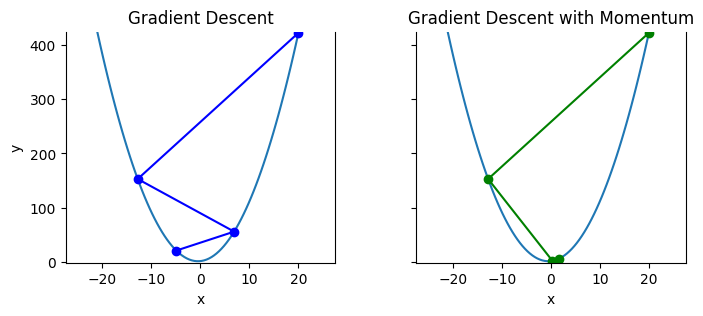
\includegraphics[width=0.45\textwidth]{report/figures/GD_momentum.png}\\
The figure illustrates, on the left, how conventional gradient descent converges towards the minimum of the depicted quadratic function. On the right, one can observe gradient descent enhanced with momentum. Although the initial step is similar for both methods, the subsequent steps differ markedly. In the case of gradient descent alone, only the current gradient is considered as the slope. However, when employing gradient descent with momentum, the direction for the next step is determined by an accumulation of the current gradient and the previous gradients, resulting in a steeper descent as the first gradient slopes upwards.\\
In ADAM the learning rate is manipulated via the first moment estimate. The biased form is defined as $$m_t=m_{t-1}\cdot \beta_1 + g_t\cdot (1-\beta_1)$$

2. explain how adam uses it



\subsection{Adaptive Learning Rate}
1. explain adaptive learning rate
2. explain how adam utilizes it
To potentially escape local minima, ADAM utilizes an adaptive learning rate method, similar to the AdaGrad optimizer. Therefore the updated biased second raw moment estimate is being utilized. Which is defined as vector $v_t$.\\

The so called $2^{nd}$ moment is calculated as:
$$v_t = v_{t-1} \cdot \beta_2 + g_t^2 \cdot (1-\beta_2)$$

This represents the moving average of the biased uncentered variance of the gradient.\\
The principle to know here is that the larger the last gradients of a certain weight value is, the smaller that weight's learning rate is going to be. Meaning that the higher $v$ the smaller the step size, because the loss function is more sensetive at this point. On the other hand the lower $v$ the bigger the step size, because the loss function is less sensetive at this point.\\
The vector $v_t$ is inizalized as $v_0$ being a vector of zeros. This creates biases, to remove the bias $v_t$ in every step is corrected as the following:
$$\hat{v_t}=\frac{v_t}{1-\beta_2^t}$$
Details for bias correction can be found in the intial paper \textit{ADAM: A Method for Stochastic Optimization} from 2015.

\subsection{The algorithm}
\begin{algorithmic}
    \If{$i\geq 5$} 
        \State $i \gets i-1$
    \Else
        \If{$i\leq 3$}
            \State $i \gets i+2$
        \EndIf
    \EndIf 
\end{algorithmic}







%PRATICAL EXAMPLE
\section{Computational Implementation}
Do a classification.  
Get an example with neural network. Use a general architecture. Maybe image classification (3Blue one Brown, video example).
\subsection{Hyperparameters}
Explain the hyperparameters that can be chosen, when each is effectfull
\subsection{Example Impleementation}
Insert Code

% COMPARISON of performance
\section{Performance Comparison}

 
\section{Conclusion}
Ending




% CODE FOR APPENDIX
\onecolumn
\newpage
\pagestyle{fancy}

\section{Appendix A}
\section*{Intuitive Explanation of ADAM}
Imagine you're playing a video game where you need to find a treasure hidden deep within a maze. The maze is foggy, so you can't see the whole layout from where you are. Your goal is to find the treasure in the least amount of time, with some areas being slippery or uphill, making your journey tougher or easier based on where you step. Here's how ADAM helps you navigate this challenge, akin to how it helps a machine learn

\subsubsection*{The Basics of Moving Around}
In this game, you have a magic map (the algorithm) that helps you decide every move (how to adjust the model's parameters) to get to the treasure (minimize the error in predictions).

\subsubsection*{Remembering Your Steps}
As you start moving, you realize that some paths you took were really good, making it easier to move forward, while others were not so great. ADAM, like a smart assistant, remembers these steps. It keeps track of your recent moves, emphasizing the better ones (this is similar to the "momentum" part of ADAM, which helps to keep moving in a good direction based on past gradients).

\subsubsection*{Adjusting Your Pace}
Some parts of the maze are slippery (easy to move fast) or uphill (hard to move). ADAM notices this and adjusts your pace accordingly. If it's slippery, it makes you take smaller steps to avoid overshooting the target, and if it's uphill, it encourages bigger steps to speed up the journey. This is like ADAM adjusting the learning rate for each parameter based on the past gradients' squared values, making sure you progress at the right speed without missing the treasure.

\subsubsection*{Getting Smarter Over Time}
The magic map gets better the longer you use it. It learns from every step you've taken, making smarter suggestions about which direction to go next. This is akin to how ADAM corrects its estimates to become more accurate over time, ensuring that the adjustments it suggests for your steps (the learning rates) are getting more and more effective.  
   
\subsubsection*{Finding the Treasure}
By remembering the good paths, adjusting your pace based on the terrain, and getting smarter over time, ADAM helps you navigate the maze efficiently and find the treasure faster than if you were just wandering around or using a less sophisticated map. This is similar to how ADAM optimizes a machine learning model's parameters to make accurate predictions or decisions, effectively "finding the treasure" in the form of the best solution to a problem. 
  
In summary, ADAM is like a highly intelligent guide for navigating through complex challenges, helping you reach your goal efficiently by learning from past experiences and adjusting your approach as you go.

\section{Appendix B}
\centering Source Code
All Notebooks and Visualizations including detailed code can be found in our GITHUB Repository with the link: \href{https://github.com/jakthehut/ADAM-Optimizer}{https://github.com/jakthehut/ADAM-Optimizer}


\end{document}